\documentclass[../../../../main.tex]{subfiles}

\begin{document}

\section*{第1問}

\begin{proof}[解]
\[
0<a<1 \quad\cdots\text{①}, \qquad 0<c\le b
\]
$f(x)=x^3+ax^2+bx+c$とおく。$f(x)=0$の3実解を$x=\alpha,\beta,\gamma$とおとき（$\alpha\le\beta\le\gamma$），$f(x)=(x-\alpha)(x-\beta)(x-\gamma)$とかけるので，係数比較して，
\[
a=-(\alpha+\beta+\gamma), \qquad b=\beta\gamma+\gamma\alpha+\alpha\beta, \qquad c=-\alpha\beta\gamma
\]
①に代入して
\[
-1<\alpha+\beta+\gamma<0 \quad\cdots\text{②}
\]
\[
\alpha\beta\gamma<0 \quad\cdots\text{③}
\]
\[
0\le\beta\gamma+\gamma\alpha+\alpha\beta+\alpha\beta\gamma \quad\cdots\text{④}
\]
③と$\alpha<\beta<\gamma$より，$\alpha<0<\beta<\gamma$（⑦）か$\alpha<\beta<\gamma<0$（⑦）である。

\textbf{⑦の時}

②から，$\alpha,\beta,\gamma$がすべて負で$\alpha$が最小だから，$\alpha+\beta+\gamma>-1$かつ$\beta,\gamma<0$より$\alpha+\beta+\gamma<\alpha$，したがって$\alpha>\alpha+\beta+\gamma>-1$。よって$-1<\alpha<\beta<\gamma<0$となる。

\textbf{⑦の時（$\alpha<0<\beta<\gamma$）は以下のように不適であることを示す}

$p=\beta+\gamma,\ q=\beta\gamma$とおくと，$\beta,\gamma$は$t$の2次式$t^2-pt+q=0$の正の2実解だから，
\[
p^2-4q>0, \qquad p>0,\ q>0
\]
②，④に代入すると
\[
-1<\alpha+p<0, \qquad 0\le\alpha p+(1+\alpha)q
\]
$\alpha<0,\ p,q>0$から，これをみたす$p,q$があるには$1+\alpha>0\ \therefore\ \alpha>-1$が必要で，このもとで
\[
-1-\alpha<p<-\alpha, \qquad q\ge-\frac{\alpha}{1+\alpha}p
\]
以上を図示すると，$-(1+\alpha)<0<-\alpha<1$と$p^2-4q>0$（すなわち$q<\dfrac14p^2$）をあわせても，$-\dfrac{\alpha}{1+\alpha}p$と$\dfrac14p^2$の大小関係および$p=-\alpha$での値を調べることで，条件をみたす$p,q$の存在範囲が空集合になる。すなわちこれをみたす$(\alpha,\beta,\gamma)$は存在しない。

以上⑦⑦から，示された。
\end{proof}

\newpage

\section*{第2問}

% (原稿は空欄。行列（一次変換）の問題であり、当時未解答)

\newpage

\section*{第3問}

\begin{proof}[解]
\textbf{(1)} $\triangle ABC$の外接円の半径1として良い。$\triangle ABC$が鈍角三角形でないとき，
\[
A(1,0), \quad B(\cos\alpha,\sin\alpha), \quad C(\cos\beta,\sin\beta) \quad\left(0<\alpha<\frac{\pi}{2},\ \pi\le\beta\le\alpha+\pi\right)
\]
とおいて良い。$D$の中心を$O'$とし，$O'\ne O$と仮定する。$D$の条件から
\[
\overline{AD}\le1,\ \overline{BD}\le1,\ \overline{CD}\le1 \iff \overline{AD}^2\le1,\ \overline{BD}^2\le1,\ \overline{CD}^2\le1 \quad(\because\text{各辺}\ge0)
\]
$D(X,Y)$とおくと，
\[
(X-1)^2+Y^2\le1 \wedge (X-\cos\alpha)^2+(Y-\sin\alpha)^2\le1 \wedge (X-\cos\beta)^2+(Y-\sin\beta)^2\le1 \quad\cdots\text{①}
\]
である。3円$P,Q,R$を
\[
P: (X-1)^2+Y^2=1, \qquad Q: (X-\cos\alpha)^2+(Y-\sin\alpha)^2=1, \qquad R: (X-\cos\beta)^2+(Y-\sin\beta)^2=1
\]
で定める。$P,Q,R$の$(0,0)$での接線の方向ベクトルは各々$\begin{pmatrix}0\\1\end{pmatrix}$，$\begin{pmatrix}-\sin\alpha\\\cos\alpha\end{pmatrix}$，$\begin{pmatrix}\sin\beta\\-\cos\beta\end{pmatrix}$だから，これを図示すると下図（$\because *$）。

$P$は$Q$の左側，$Q$は$R$の上側，$R$は$P$の左側にあるから，$P,Q,R$の共有点は$O(0,0)$のみ，つまり
\[
①\iff(X,Y)=(0,0)
\]
であるが，これは$O'\ne O$に反し矛盾。以上から示された。

\textbf{(2)} (1)のベクトル図から，$\triangle ABC$が鈍角三角形になれば①の領域式が$(0,0)$以外に広がり，$D\ne O$となる。したがって，
\[
\triangle ABC\text{が非鈍角三角形}\iff D=O \quad\cdots\text{②}
\]
となる。したがって，$\triangle ABC$が鈍角三角形になるような$C$の軌跡を求めれば良い。対称性から，$0\le x,\ 0<y$で考える。又，$C(x,y)$とする。

\textbf{$1^\circ$ $1<x$の時}

$\angle CAB>\pi/2$となり，$\triangle ABC$は鈍角三角形。

\textbf{$2^\circ$ $0\le x\le1$の時}

$\angle CAB\le\pi/2,\ \angle CBA\le\pi/2$だから，$\angle ACB>\pi/2$となる条件をしらべれば良い。このような条件は
\[
x^2+y^2<1
\]
である。

以上$1^\circ,2^\circ$から，$0\le x,\ 0<y$では，題意の条件は $1<x$ or $x^2+y^2<1$だから，対称性から求める領域式は
\[
|x|>1 \ \text{または}\ x^2+y^2<1 \quad(y\ne0)
\]
であり，制約$x^2+y^2\le4$とあわせて図示して下図斜線部（境界は$x^2+y^2=4$のみ含み，$x$軸は含まず）。

\begin{center}
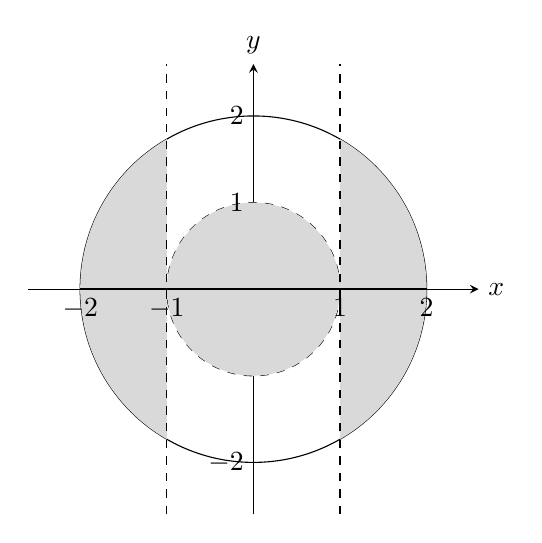
\begin{tikzpicture}[scale=1.1, >=stealth]
  \draw[->] (-2.6,0) -- (2.6,0) node[right] {$x$};
  \draw[->] (0,-2.6) -- (0,2.6) node[above] {$y$};
  \draw (0,0) circle (2);
  \draw[dashed] (0,0) circle (1);
  \begin{scope}
    \clip (0,0) circle (2);
    \fill[gray!30] (-2.6,-2.6) rectangle (-1,2.6);
    \fill[gray!30] (1,-2.6) rectangle (2.6,2.6);
    \fill[gray!30] (0,0) circle (1);
  \end{scope}
  \draw[dashed] (-1,-2.6) -- (-1,2.6);
  \draw[dashed] (1,-2.6) -- (1,2.6);
  \draw[thick] (-2,0) -- (2,0);
  \node[below] at (-2,0) {$-2$};
  \node[below] at (-1,0) {$-1$};
  \node[below] at (1,0) {$1$};
  \node[below] at (2,0) {$2$};
  \node[left] at (0,2) {$2$};
  \node[left] at (0,1) {$1$};
  \node[left] at (0,-2) {$-2$};
\end{tikzpicture}
\end{center}
\end{proof}

\newpage

\section*{第4問}

\begin{proof}[解]
$x(t)=t+e^{at},\ y(t)=-t+e^{at}$とおく。又，$p=e^t$とする。
\[
x'(t)=1+ap^a, \qquad y'(t)=-1+ap^a \quad\cdots\text{①}
\]
$a>0$から，$x'(t)>0$だから
\[
\frac{dy}{dx}=\frac{y'(t)}{x'(t)}=\frac{-1+ap^a}{1+ap^a} \quad\cdots\text{②}
\]
題意から，$y(t)=0$の時，$dy/dx=0$なる$t$がある。$dy/dx=0\iff a\cdot p^a=1$（$\because②$）で，これをといて，（$a>0$）
\[
t=-\frac1a\log a
\]
この時$y(t)=0$となるから，
\[
\frac1a\log a+\frac1a=0 \quad\therefore\ a=\frac1e\ (>0)
\]

\textbf{(2)} ②及び(1)の結果から下表をうる。
\begin{center}
\begin{tabular}{c|ccccc}
$t$ & & & $e$ & & \\
\hline
$x'$ & $+$ & $+$ & $+$ & & \\
\hline
$y'$ & & $-$ & $0$ & $+$ & \\
\hline
$(x,y)$ & $\searrow$ & & $(2e,0)$ & & $\nearrow$
\end{tabular}
\end{center}
$t\to+\infty$の時，$x(t),y(t)\to+\infty$。$t\to-\infty$の時，$x(t)\to-\infty,\ y(t)\to+\infty$。
\[
x(t)\le y(t)\iff t+e^{t/e}\le-t+e^{t/e}\iff t\le0 \quad(x(0)=1,\ y(0)=1)
\]
とあわせて，グラフの概形は下図でもとめる面積$S$は下図斜線部。

\begin{center}
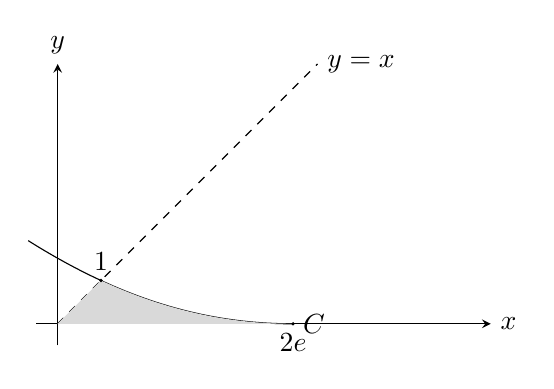
\begin{tikzpicture}[scale=0.55, >=stealth]
  \draw[->] (-0.5,0) -- (10,0) node[right] {$x$};
  \draw[->] (0,-0.5) -- (0,6) node[above] {$y$};
  \draw[dashed] (0,0) -- (6,6) node[right] {$y=x$};
  \draw[domain=-1.3:2.72, smooth] plot ({\x+exp(\x/2.71828)},{-\x+exp(\x/2.71828)}) node[right] {$C$};
  \fill[gray!30] (0,0) -- (1,1) -- (1,0) -- cycle;
  \fill[gray!30, domain=0:2.71828, variable=\tau] plot ({\tau+exp(\tau/2.71828)},{-\tau+exp(\tau/2.71828)}) -- (1,0) -- cycle;
  \fill (1,1) circle (1.2pt) node[above] {$1$};
  \fill (5.436,0) circle (1.2pt) node[below] {$2e$};
\end{tikzpicture}
\end{center}

\[
S=\triangle+\int_1^{2e}y(t)dx=\frac12+\int_1^{2e}y(t)dx=\frac12+\int_0^ey(t)\frac{dx}{dt}dt \quad\cdots\text{③}
\]
ここで，
\[
y(t)\frac{dx}{dt}=\left(-t+e^{\frac{t}{e}}\right)\left(1+\frac1ee^{\frac{t}{e}}\right)=\frac1ee^{\frac2et}+\left(1-\frac{t}{e}\right)e^{\frac{t}{e}}-t \quad\cdots\text{④}
\]
であり，各項計算して，
\[
\int_0^e\frac1ee^{\frac2et}dt=\frac12\left[e^{\frac2et}\right]_0^e=\frac12(e^2-1)
\]
\[
\int_0^e\left(1-\frac{t}{e}\right)e^{\frac{t}{e}}dt=e\int_0^1(1-x)e^xdx=e^2-2e
\]
\[
\int_0^et\,dt=\frac12e^2
\]
だから④に代入して，
\[
④=\frac12(e^2-1)+e^2-2e-\frac12e^2=e^2-2e-\frac12
\]
だから，③から
\[
S=e(e-2)
\]
\end{proof}

\newpage

\section*{第5問}

\begin{proof}[解]
\textbf{(1)} $k+l$回の移動のうち，行何回目に上へ移動するかかんがえて，
\[
P(k,l)={}_{k+l}C_k\left(\frac12\right)^{k+l}
\]

\textbf{(2)} 右図から
\[
P(n,2)=P(n,1)+\frac12P(n-1,2) \quad\cdots\text{①}
\]
\[
P(n,1)=P(n,0)+\frac12P(n-1,1) \quad\cdots\text{②}
\]
ここで，$P(n,0)=\left(\dfrac12\right)^n$，$P(n-1,2)={}_{n+1}C_2\left(\dfrac12\right)^{n+1}$，$P(n-1,1)={}_nC_1\left(\dfrac12\right)^n$（$\because(1)$）だから②，①に代入して
\[
P(n,1)=\left(\frac12\right)^n+\frac{n}{2}\left(\frac12\right)^n
\]
\[
P(n,2)=\left(1+\frac{n}{2}\right)\left(\frac12\right)^n+\frac12\cdot\frac{(n+1)n}{2}\left(\frac12\right)^{n+1}
\]
\[
=\frac{n^2+5n+8}{8}\left(\frac12\right)^n
\]
\end{proof}

\end{document}
